\documentclass[10pt]{article}
\usepackage{graphicx}
\usepackage{xcolor}
\usepackage{caption}

\title{Figures for manuscript}
\date{April 29, 2026}
\author{}

\begin{document}

\noindent
Hey guys we wanted to ask some questions about the theory to get a better understanding of what additional things to try in the lab.\\
Also regarding your inquiry about draft format: Attached below are the two figures (Figure \ref{cs2_jet_vs_droplet} and two options for Figure 2) we are planning on showing in the paper. For both figures there is a short description of the main punchline/ the key result we want to state and some preliminary information in the caption. This might give you a rough guideline. Please feel free to comment on this as well. 
\newline
\vskip 10pt
\noindent
\textbf{General questions regarding the theory:}
\begin{itemize}
    \item \textbf{Question 1:} We are curious how your simulation results depend on the acceleration of the centrifuge. Is each time step in your simulation calculated independently? On slides 15-21 it seems like $\Omega$ has no time dependence and you say the Hamiltonian in the rotating frame is time-independent, but then on slide 24 you say "Solving for eigenstates with V(t) and $\Omega(t)$". How we currently understand your theory there would be no difference between a decelerating and accelerating centrifuge (meaning the $cos^2$ plot would just be mirrored)? 
    \item \textbf{Question 2:} On slide 21, for the case of fast relaxation, do you mean to say that we recover $\rho_0$ at each time step (which would correspond to a different field polarization/molecular alignment direction)? In that regard can you define again what $t_{bath}$ is?
\end{itemize}
\vskip 20pt
\textbf{Questions regarding the simulations:}

\begin{itemize}
    \item \textbf{Question 3:} Can you explain why the lower envelope of the simulated $CS_2$ $cos^2\theta_{\mathrm{2D}}$ signal doesn't look comparable to our empirical data? That is to say, the oscillations don't have minima going down to a constant baseline (like 0.5) in your simulation. Whereas the lower baseline for the simulated OCS agrees with our measured data. Might that be because you're using $10^{10}\, \frac{W}{cm^2}$ instead of our nominal $10^{12}\, \frac{W}{cm^2}$ for the peak intensity? 
\end{itemize}
\vskip 10pt
Comment - If it's not too much work, would it be possible for you to share your simulation program with us? Do you have it saved as a repository on GitHub? \\\\
Either way, could you send the .csv files from the plots you made so far so that we can incorporate them into the figures.

\newpage
\begin{figure}
\centering
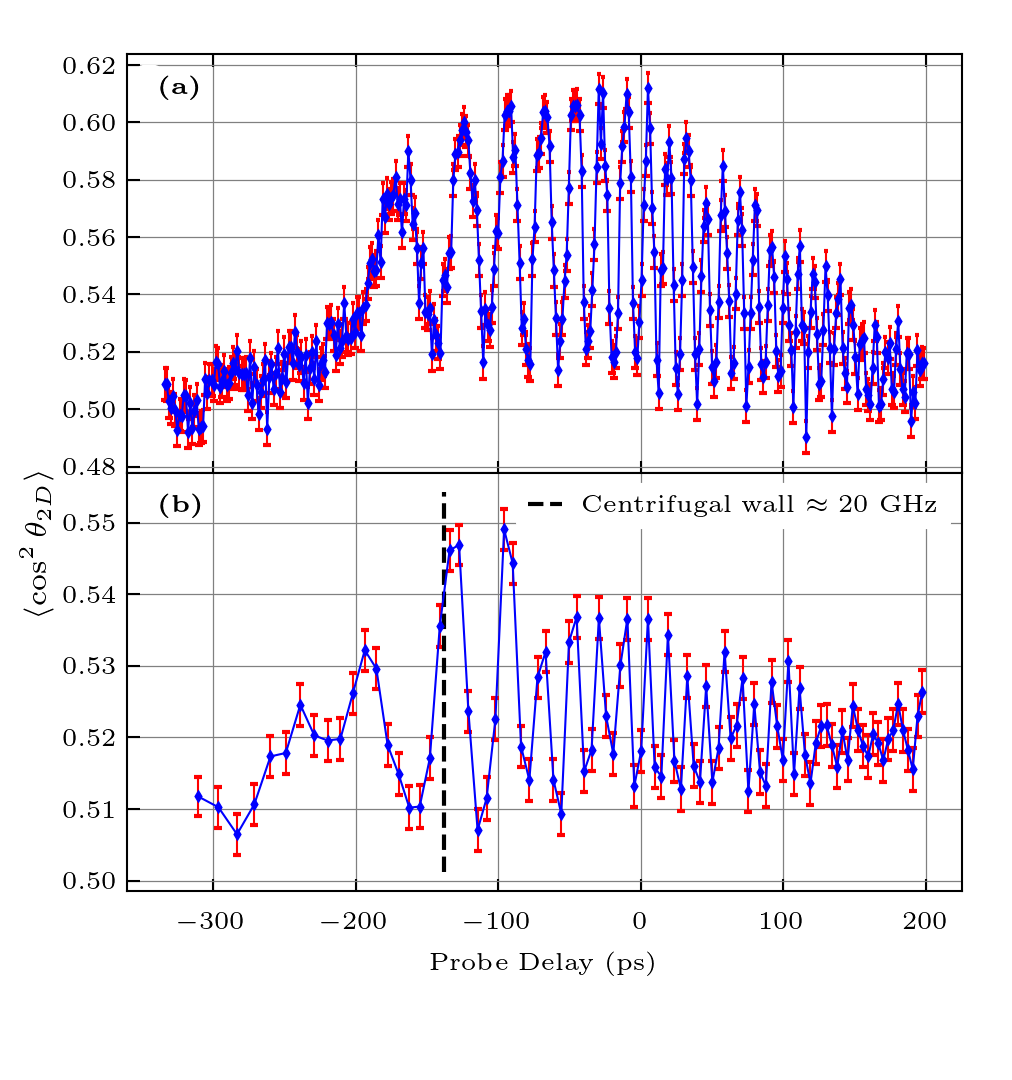
\includegraphics{cs2-breakingwall.png} 
\caption{Molecular alignment of gas-phase CS2 \textbf{(a)} and CS2 molecules embedded in He droplets \textbf{(b)} to the same phase-stabilized centrifuge. }
\label{cs2_jet_vs_droplet}
\end{figure}
\noindent
\textbf{Comments on figure 1:}
\begin{itemize}
    \item with the centrifuge we are able to spin molecules in helium past the centrifugal wall $\rightarrow$ for CS2 the wall is at around $20 \, GHz$
    \item compared to the free rotating molecules in the gas-phase there seems to be a decrease in oscillation amplitude after $-100 \, ps$ corresponding roughly to $30-40\, GHz$
    \item 
\end{itemize}

\newpage
\begin{figure}[h]
\centering
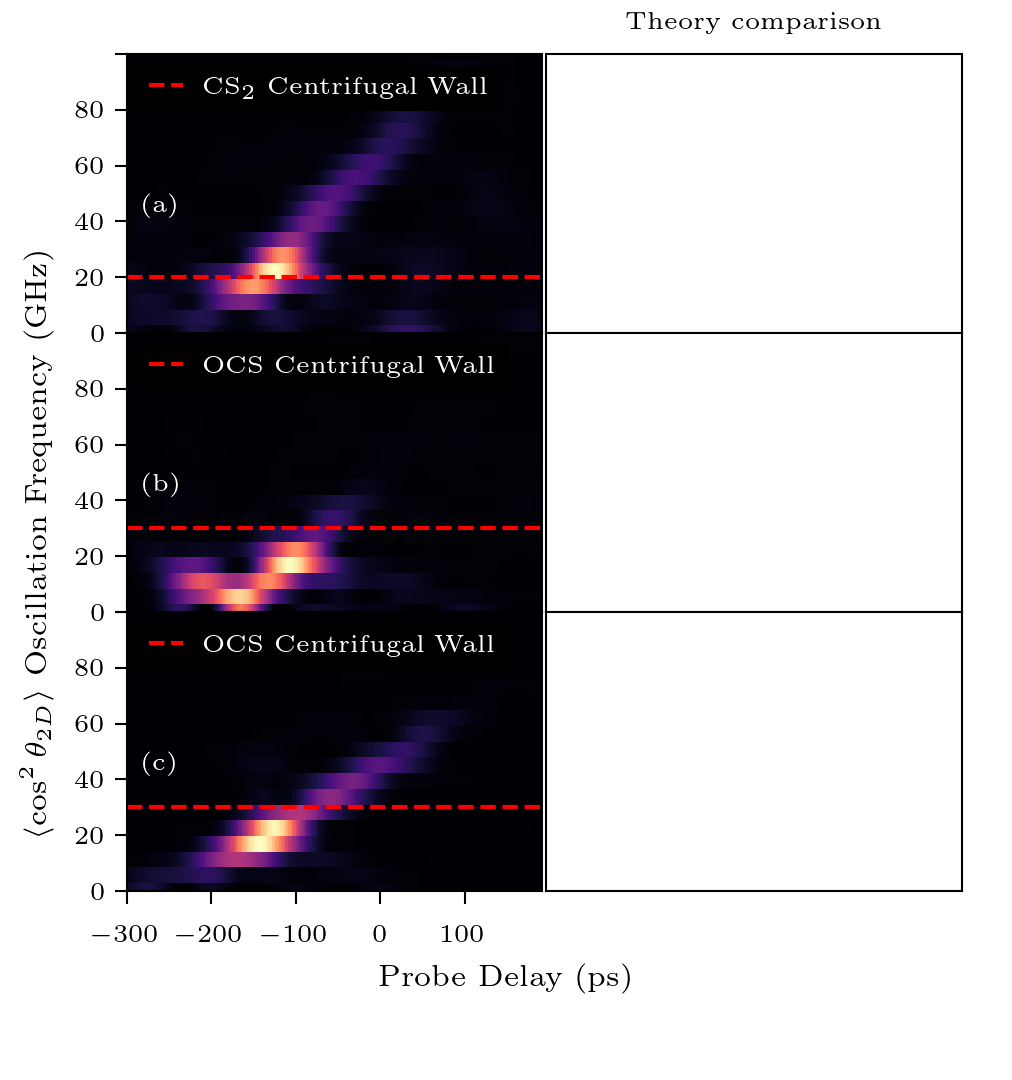
\includegraphics{cs2-ocs-comparison_v1.png}
%\captionsetup{name = Figure 2 [option 1],labelsep=newline}
\caption*{Figure 2 [\textbf{option 1}]: STFT of the experimental (left panel) and theoretical (right panel) $\langle\cos^2\theta_{\mathrm{2D}}\rangle(t)$ signal of molecular rotation in helium droplets of CS\textsubscript{2} \textbf{(a)} and OCS \textbf{(b)} with a higher centrifuge acceleration ($\approx 0.34$ GHz/ps), and OCS \textbf{(c)} with a lower centrifuge acceleration ($\approx 0.26$ GHz/ps). Note that the centrifuge used in \textbf{(b)} decelerates in the beginning of the pulse before reaching 0 GHz and then accelerating. This is reflected in the corresponding spectrogram \textbf{(b)} from about -250 ps to -150 ps.}
\label{cs2_vs_ocs_v1}
\end{figure}
\begin{figure}[h]
\centering
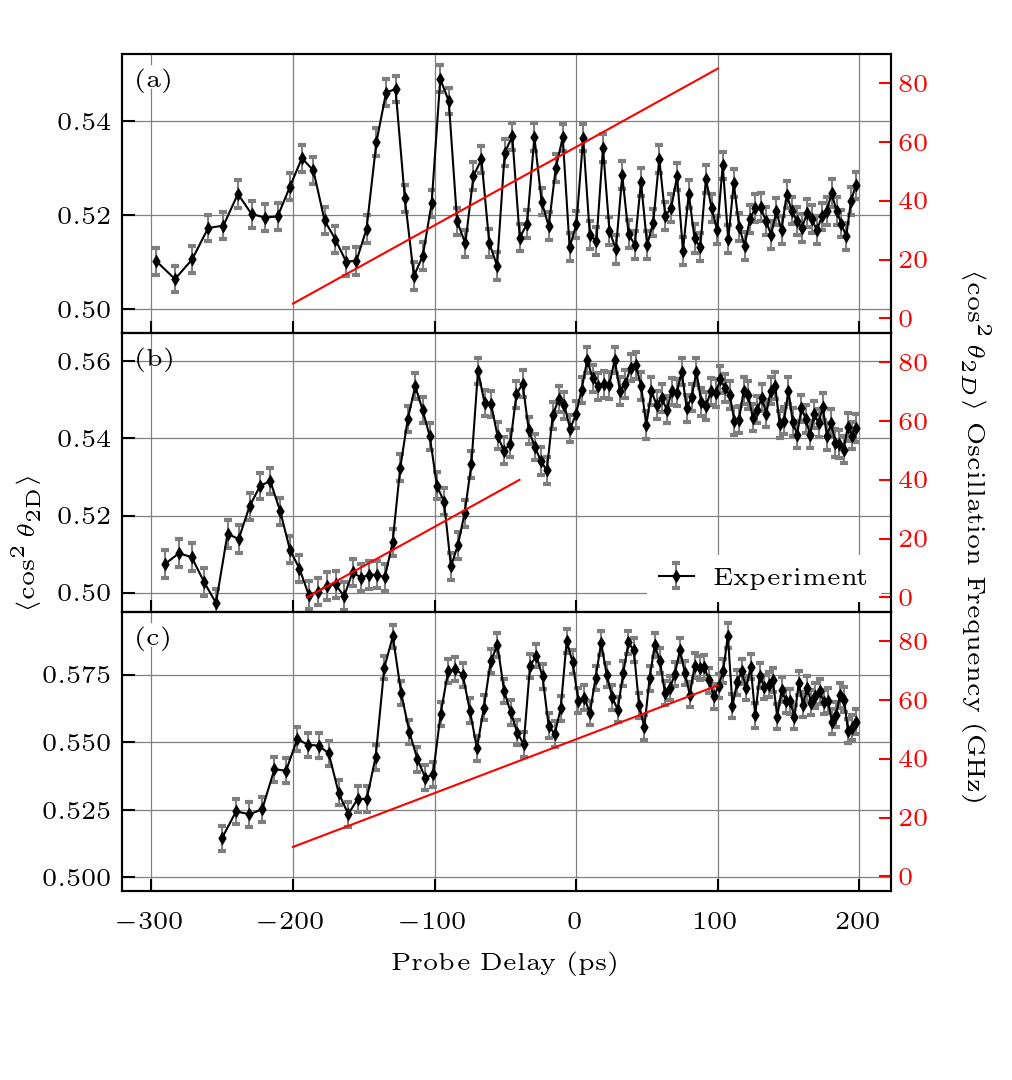
\includegraphics{cs2-ocs-comparison_v3.png}
%\captionsetup{name = Figure 2 [option 2],labelsep=newline}
\caption*{Figure 2 [\textbf{option 2}]: Molecular alignment (experimental curve to be overlaid with theoretical curve) of CS\textsubscript{2} \textbf{(a)} and OCS \textbf{(b)} with a higher centrifuge acceleration ($\approx 0.34$ GHz/ps), and OCS \textbf{(c)} with a lower centrifuge acceleration ($\approx 0.26$ GHz/ps). The truncated lines plotted with respect to the right axes represent the best linear fits (only by eye for now) to the STFTs of the $\langle\cos^2\theta_{\mathrm{2D}}\rangle(t)$ curves. Note that the centrifuge used in \textbf{(b)} decelerates in the beginning of the pulse (-250 ps to -150 ps) before reaching 0 GHz and then accelerating.}
\label{cs2_vs_ocs_v3}
\end{figure}
\newpage

\noindent
\textbf{Comments on figure 2:}
\begin{itemize}
    \item this plot compares two different molecules (CS2 and OCS)
    \item we see that in case of the faster accelerating centrifuge oscillations persist further for CS2
    \item lowering the acceleration makes it possible to see oscillations in OCS till at least $60\, GHz$ $\rightarrow$ again way above the centrifugal wall predicted for OCS
    \item ------------------------------------------------------------
    \item the comparison to theory should be included in this figure either by showing the spectrograms (option 1) or by plotting the rescaled theoretical $cos^2$ scans (option 2)
\end{itemize}
\end{document}